\documentclass{UoYCSproject}
\usepackage{booktabs}
\addbibresource{dummyBib.bib}
\author{Katie Maison}
\title{Supporting Software Development Planning with a BERT-Based Ticket Estimation Model}
\date{2nd May 2024}
\supervisor{Peter Nightingale}
\BSc
 \usepackage{rotating}
 \usepackage{tabularray}

\let\oldenumerate\enumerate
\let\endoldenumerate\endenumerate
\renewenvironment{enumerate}{\oldenumerate\setlength{\itemsep}{0pt}\setlength{\parskip}{0pt}\setlength{\parsep}{0pt}}{\endoldenumerate}

\acknowledgements{
  I would first like to thank my supervisor, Peter Nightingale, for his guidance and support throughout this project. \par
  I would also like to thank my family for their support and encouragement, and my son Alfie and partner Alex for their endless patience and love.
}

% More definitions & declarations in example.ldf
\begin{document}
\pagenumbering{roman}
\maketitle
\listoffigures
\listoftables
%\usepackage{booktabs}

%\renewcommand*{\lstlistlistingname}{List of Listings}
%\lstlistoflistings
    \begin{summary}
        With the rise of Agile software development, the estimation of tickets has become an integral part of project planning.
        Project planning is a key way of ensuring that a project is delivered on time, and that the work is prioritised correctly.
        The model proposed in this paper is a step towards automating the estimation of tickets, and could be used to improve the overall accuracy and speed of the estimation process in software development projects.\par

        In this project, I propose a model that uses a large language model to classify tickets into 3 categories, “Small”, “Medium” and “Large”.
        The model uses the title and description of the ticket as input features, and is trained on a dataset of 19,500 tickets from a large automotive company.
        The base of the model is a Bidirectional Encoder Representations from Transformers (BERT) model, which is a large language model that is designed to understand and generate human language.
        The model is fine-tuned on the dataset using a classification neural network, and is evaluated on its accuracy and training time.

        The model proposed in this paper aims to achieve an accuracy of 70\% or higher, to be useful in the estimation process.
        The model is also required to take less than 4 hours to train, and be able to classify tickets in less than 10 seconds. \par

        The proposed solution achieved an accuracy of 73.5\% on the test set, took 3 hours and 45 minutes to train, and is able to classify tickets in less than 2 seconds.
        The model is also tested on a set of tickets from an internal Platform team project rather than embedded automotive system tickets that were used for training, achieving an accuracy of 44\%.

        In this paper I also propose ways that the model could be used in practice, including as an advisor for the “expert” who is estimating tickets, or as a participant in planning poker sessions with members of a project.
        A hosting solution is also proposed, where the model could be hosted on an cloud service and accessed via an API from a ticketing system such as Jira, allowing for real-time classification of tickets. \par

        Further work could include training the model to output a time or story point estimate rather than a category, as this would be more useful in practice.
        This may require more data or a different model architecture.
        Another area of improvement that could be explored is the use of a multilingual model, as the model proposed in this paper is only trained on English text. \par

        Ethical considerations are also discussed in this paper, including the risk of bias in the model, and the importance of ensuring that the model is not used to estimate tickets without human oversight. The risk of bias in the model is mitigated by removing gendered pronouns and names from the dataset, and by ensuring that the model is not used to estimate tickets without human oversight.
        As the dataset used in this project is from a large automotive company, permission has been sought from the company to use the data, and the data has not been made public to ensure that no sensitive information is leaked.
        I have not sought approval from the ethics committee as the topic of the project is not sensitive, and the data has been anonymized.
        \par


    \end{summary}

    \chapter{Introduction}
    \label{ch:introduction}
    \setcounter{page}{1}
    \pagenumbering{arabic}


    Late delivery of software projects remains an ever-present challenge, often attributed to the inherent uncertainties and complexities associated with development.
    Multiple factors affect the delivery of a software project, however, it is clear that project planning plays a role in this~\cite{CHOW2008961}. \par
    Agile Software development is a type of iterative planning method where a project is broken up into smaller “user stories” or tickets, each defining a specific task or part of a project that must be completed.
    It was introduced in 2001 by a group of software developers who wanted to move away from the traditional “waterfall” method of software development, where a project is planned in its entirety before any work is carried out, to a more iterative and flexible method of development~\cite{beck2001agile}.
    Generally, each ticket has an estimate attached to it, defining the time or effort it will take to finish.
    Some projects use time-based estimates like hours or days to estimate tickets, others teams assign “Story Points”, an abstract unit of perceived complexity, risk, and effort involved in implementing a specific feature or piece of functionality.
    It is common for the Story Point scale used to be a modified Fibonacci, of 1, 2, 3, 5, 8, 13, 15, 20, 40, 100 \cite{scrumFib}.
    A ticket that is estimated to be 1 Story Point is deemed to be the smallest amount of work that can be done, and a ticket that is estimated to be 100 Story Points is deemed to be the largest amount of work that can be done.
    A 1 story point ticket would be something a developer would consider relatively easy, requiring minimal effort to complete, most likely less than an hour or active work.
    Therefore a 2 story point ticket would be something that would require double the amount of effort and may take double the amount of time, although something could take a small amount of effort and a longer time to complete due to having to wait for builds or similar.
    This would still count as a 1 or 2 story point ticket as the effort is being estimated rather than the time.
    Estimates enable a Team leader to plan what tickets can be completed in a “sprint”, or “iteration”, usually a period of 2-4 weeks, based on how many points they think the team will be able to do.
    The number of story points that a team can complete in a single iteration is known as the teams `Velocity'~\cite{cohn2005agile}.
    The process for estimating tickets can be time consuming, the faster that a ticket is estimated, the faster it can be planned for completion.
    Furthermore, the more accurate an estimation is, the more likely it is that a release can be delivered on time, as the work will have been planned accordingly.
In agile development, a release is a collection of tickets associated with features or bug fixes due to be added to a product. \par

    When a ticket is created, it is placed into a to-do list of tickets called a `backlog'.
    Tickets in the backlog are then estimated for their effort or time to complete, and are then ordered according to multiple factors including this estimate and the priority of the ticket.
    Generally in projects, work cannot be carried out on a ticket until it has been estimated.
    This emphasises the importance of both the speed and accuracy of ticket estimation in the successful management of projects.
    Automated ticket estimation may enable the correct prioritisation of tickets before any estimation activities are carried out by the team or members of the team. \par

    In this project, I use a machine learning approach to automate the estimation of tickets.
    By using a large language model, the information provided in a tickets title and description can be used as features in a classification neural network.
    The model proposed in this paper is intended to participate in the estimation process rather than perform the estimation as the source of truth.
    This is because incorrect estimates can have severe consequences on project planning, a model would need to be extremely accurate to be trusted to estimate the ticket correctly.
    In practice the model participation can happen in multiple ways.
    The model may act as an advisor for the “expert” who is estimating tickets.
    Alternatively, the model may participate in planning poker sessions with members of a project.
    Planning poker is when engineers play a “game” where everyone chooses a card that equates to the value that they want to estimate, then discuss and re-estimate until a consensus is reached~\cite{1667560}. \par

    To simplify the problem, the model proposed in this paper will be able to classify tickets into 3 categories, “Small”, “Medium” and “Large”.
    When inspecting data from a project in a large automotive company, who estimate using minutes and hours, it was found that the accuracy of ticket estimation was 74\% when using the above categories. I also looked at the speed
    Therefore, I am setting the following objectives for the model:
    \begin{enumerate}
        \item To classify tickets into 3 categories, “Small”, “Medium” and “Large” with an accuracy of 70\% or higher.
        \item To ensure that the model takes less than 4 hours to train.
        \item To be able to classify tickets in less than 10 second.
    \end{enumerate}

    Objective 2 is so that the model can be retrained on a regular basis to ensure that it is up to date with the latest data, ensuring continuous learning but also reduce costs.
    Objective 3 is so that the model can be used in real time, for example in a planning poker session, where the model can be used to classify tickets as they are being discussed.


    \chapter{Literature Review}
    \label{ch:literature-review}
    This section discusses the current research into methods of ticket estimation, including with Deep learning, as well as in the broader field of Natural Language Processing.
    It summarises and analyses existing work as well as highlighting unknowns within the topics.

    It is broken down into three sub-sections.
    First “Estimation in Software Engineering Projects” focuses on research about effort and time estimation as a concept, as well as research into techniques for doing estimations.
    The next sub-section focuses on relevant research into Large Language Models and Natural Language Processing.
    Lastly, the “Agile Estimation with Deep Learning” looks at Deep learning models specifically for classification of text, particularly of Agile Tickets for estimation.


    \section{Effort Estimation}
    \label{sec:effort-estimation}
    Current research into estimation in agile projects mostly centres around how estimations are produced and what scale they use.
    There are many methods for estimating tickets or projects that have been examined in academic research.
    They can be sorted into two main categories, Judgement-based approaches and Model-based approaches (discussed below).

    \subsection{Judgement-based approaches}
    \label{subsec:judgement-based-approaches}

    Judgement-based approaches rely on the knowledge of experts about the field or project in question, who can make an estimate based on their experiences and knowledge on how much effort a ticket will take to complete.
    The simplest judgement based approach, expert judgement, is a single expert estimating the ticket by themselves.
    Group or Team estimation techniques such as Planning poker, whereby team members play a “game” to reach an agreement on the Story Point estimate of a tickets are also popular.
    Research has been done to examine the accuracy of these techniques by looking at the result of the same ticket estimated with both, showing that planning poker is more accurate than individual expert estimates~\cite{MAHNIC20122086, RashidSCE}. \par
    In 2015, a survey was performed to determine the state of the practice of Effort Estimation of Agile Software Development, claiming to be the first of its kind.
    The research surveyed 60 users of agile practices across 16 different countries.
    It asked which estimation techniques each person uses at their work.
    Of the participants, 52\% selected multiple estimation techniques.
    The survey found that 63\% of participants use Planning poker to perform estimations followed by 47\% who use Analogous estimation (whereby parallels are drawn from previous stories and they are used to decide an estimate for new stories) and expert judgment (38\%)~\cite{effortestimationsurvey}.
    The servey also found that the most common scale used for estimation was story points, with 61\% of participants using it.
    Only 21\% of participants believed that their estimation techniques were accurate to within 5\% of the actual effort required to complete a ticket.
    The survey also examined peoples beliefs on reasons for inaccurate estimations, with 32\% saying that it is due to inaccurate or changing requirements and poorly written tickets.
    Other reasons were Project Management issues (25\%), Team related issues such as lack of knowledge or experience (18\%) and overoptimism, lack of formal estimation process, ignoring testing effort and insufficient customer involvement at $\leq 10$\% each.
    Unfortunately although responses were collected from 60 different people, the survey does not report how many companies responses were collected from. This may call in to question the validaty of the data for the wider agile community. \par
    \subsection{Model-based approaches}\label{subsec:model-based-approaches}
    In the last 30 years, many Algorithmic-Based Approaches have been proposed to automate the estimation of software development projects.
    In 1981, the Constructive Cost Estimation Model ($COCOMO$) model was proposed by DR. Berry Boehm~\cite{Boehm2001}.
    The basic $COCOMO$ model defines the effort required to complete a project to be $a^2 \times (KLOC)a^2pm$.
    Where $KLOC$ is kilo lines of code, $a$ is a constant depending on the type of project and is expressed in person months ($pm$). The detailed version adds effort multipliers for each phase of a project, splits the effort estimation into subsystems and adds various extra multipliers to improve accuracy.
    Although this model can achieve a mean average accuracy of 91\% for effort estimation on projects, the model requires a lot of input information, including Lines of Code, number of files, number of external interfaces and developer experience with the technical stack.
    COCOMO, as well as other model based estimators and regression models, are used much less in agile software development than previously in non-agile development methods.
    This is likely due to the estimations in agile being for tickets rather than for entire projects, where the attributes needed are more readily available and relevant and the planning stages are more extensive~\cite{effortestimationsurvey}.
    With the shift towards agile software development, focus has shifted towards researching how we can leverage Natural Language Processing in order to estimate story points.



%    https://ieeexplore.ieee.org/stamp/stamp.jsp?tp=&arnumber=4343762 TODO

    \section{Large Language Models}
    \label{sec:large-language-models}
    Large Language Models (LLM) are a type of artificial intelligence model that is designed to understand, generate
    or manipulate human language.
    These models are characterized by their size and complexity, often consisting of millions or even billions of parameters.
    Large language models are built on advanced deep learning architectures and are typically pre-trained on massive amounts of textual data (corpus) before being fine-tuned for specific tasks. \par

    In 2017, transformer based architecture was introduced in a model proposed by Vaswani et al.
    in their paper, ``Attention is all you need''~\cite{vaswani2023attention}.
    It has become the foundational model for a variety of natural language processing (NLP) tasks, including text classification, question answering, summarization, and translation.
    The transformer based architecture is a type of neural network architecture that is designed to process sequential data, such as text, and is based on the concept of attention.
    The core innovation of this architecture is the introduction of `self-attention'.
    Self-attention allows a model to weigh the importance of different words in a sequence when processing each word, rather than relying on a fixed-length context window, like in recurrent neural networks (RNNs) \cite{RNNbook}.
    It also allows the model to process all words in a sequence simultaneously, rather than sequentially, therefore improving the training speed as it allows parallelization.
    The mechanism computes attention scores for each token in the input sequence, indicating how much attention should be paid to other tokens.
    By considering relationships between all tokens simultaneously, the model can capture long-range dependencies and contextual information effectively.
    To capture diverse types of information and relationships, the self-attention mechanism is typically divided into multiple attention heads.
    Each head independently computes attention scores, allowing the model to focus on different aspects of the input.
    By combining information from multiple heads, the model can capture a richer set of features and relationships within the sequence.
    \par
    In June 2018, Generative Pre-Trained Transformers (GPT) was introduced by OpenAI in the paper ``Improving Language Understanding by Generative Pre-Training''~\cite{GPT2018}.
    GPT follows an autoregressive approach during both pre-training and fine-tuning, this means that the model generates text sequentially, predicting the next word in a sequence based on the preceding context.
    This allows GPT to capture complex dependencies and relationships in language, however GPT only looks at the context of previous words, left-to-right rather than bidirectionally like later models.
    GPT achieved a GLUE benchmark score of 72.8\% on average, outperforming previous state-of-the-art models at the time of 68.9\% .
    GLUE was introduced in "GLUE: A Multi-Task Benchmark and Analysis Platform for Natural Language Understanding" in 2018 ~\cite{wang2019glue}.
    It is a collection of test sets for evaluating and comparing the performance of models across a diverse range of NLP tasks, including sentiment analysis, question answering, and text classification.

    \par

    In the years since the initial GPT release, openAI has released multiple versions of the model, with the most recent at time of writing being GPT-4 which was released in 2023~\cite{openai2024gpt4}.
    OpenAI did not test GPT-4 on the GLUE benchmark.
    They did however test it on some standard exams originally designed for humans, which achieved results above the 80th centile in many, including the Uniform Bar Exam (~90th centile) and SAT Math (~89th centile). It got much lower scores in AP English Language and Composition (8-44th centile)  \cite{openai2024gpt4}.
    The GPT paper says that to check whether the questions in the exams were present in the training data, they only employed a random sampling of substrings from questions and checked them against the training data.
    This means that there is a chance that the questions in the exam papers were present in the GPT Training set, which would make it an unfair test.
    Furthermore, there are various concerns and skepticism around the performance of the model on the Bar exam \cite{Sullivan2024-bk, EvalBarGPT}.
    The National Conference of Bar Examiners (NCBE) mandates that bar exam graders be trained in bar exam grading, however although some of the researchers involved in the study were lawyers, the paper does not state that any were trained in Bar exam grading.
    Instead the answers were compared to a number of "good answers" from test-takers in Maryland.
    This calls into question these results, which got the most publicity of all the results described in the paper. \par

    \par

    In October 2018, the Bidirectional Encoder Representations from Transformers (BERT) model was introduced by Devlin et al~\cite{devlin2019bert} .
    BERT is a large language model that uses the transformer architecture and is pre-trained on a large corpus of unlabelled text, including the entire Wikipedia corpus and a large book corpus, totaling 3,300M words.
    It is trained using a masked language model (MLM) objective, where random tokens in a sequence are masked, and the model is trained to predict those masked tokens.
    BERT is considered a landmark in the development of large language models, for multiple reasons.
    An important difference between BERT and previous language models is that it is bidirectional, meaning that it can
    use the context of both the left and right side of a word when processing it, enabling the model to capture richer contextual information compared to previous unidirectional models.
    At time of release, BERT outperformed all other Large Language Models on the General Language Understanding Evaluation (GLUE Benchmark).
    An average of 79.6\% on the $GLUE$ benchmark tasks was achieved by the $BERT_{base}$, 4.4\% higher than the previous highest score achieved by OpenAI's GPT.

    The release of BERT and GPT in 2018 was followed by the proposal of many new models based on the transformer architecture in 2019.
    XLNet was introduced by researchers at Google and Carnegie Mellon University, it is another transformer-based language model that extends the bidirectional context understanding of BERT while addressing some of its limitations~\cite{yang2020xlnet}.
    XLNet uses a permutation language model (PLM) objective.
    Instead of masking random tokens, XLNet considers all tokens in the sequence as potential candidates for prediction.
    This means that the model is trained to predict the probability distribution over all possible permutations of the sequence. \par

    \section{Text Classification with Large Language Models}
    \label{sec:text-classification}
    Large language models have been shown to be effective in a wide range of natural language processing tasks, including text classification.
    Text classification is the process of assigning a label or category to a piece of text based on its content.
    It is a fundamental task in NLP and has many applications, such as sentiment analysis, spam detection, and topic classification.
    Zero shot learning in text classification is a type of training where a model is trained to classify text into categories that it has never seen before\cite{zeroshot}.
    For example a model trained on classifying animals could be used to classify a piece of text about a car, without ever seeing a car in the training data.
    This is beneficial as it allows the model to be used in a wider range of applications, without needing to be retrained for each new category.
    This technique was examined in a paper called ``Zero-shot Text Classification With Generative Language Models'', where Puri et al found that a zero shot trained model could achieve up to 45\% absolute improvement over random baselines ~\cite{puri2019zeroshot}.
    Few shot classification is a type of text classification where a model is trained on a small number of examples for each category that it will be classifying text into~\cite{luo2023closer}.
    For example, a model trained on classifying animals could be trained on a small number of examples of each animal that it will be classifying.
This method has gained popularity as it allows the model to be trained on a small amount of data, which is beneficial when data is scarce \cite{luo2023closer}.
    However in this paper, a pre trained model will be trained on a large number of examples for each category in the task, as the data is available, in order to make the model task specific.
    This is referred to as fine-tuning.
    This is a common way of training image and text classification models for many tasks, including sentiment analysis of text and Medical image classification \cite{SentAnalysis, medFineTuning}.
\par



%
% An important part of Large language models is Tokenization, which is the process of splitting a string into a list of
%    tokens.
%    A token can be a word, sentence, paragraph or even a single character.
%    Tokenization is performed by a Tokenizer, which is a class that defines a vocabulary and methods for encoding.
%    The vocabulary is a list of known tokens, for example words from a dictionary or in a particular corpus.
%    The Tokenizer can then encode a string by breaking it up into tokens and replacing each token with its corresponding integer value from the vocabulary.
%    One popular tokenizer is WordPiece, which was introduced in 2016 by Google as the tokenization method for BERT [BERT].
%    WordPiece is a sub-word tokenizer, meaning that it breaks words down into smaller parts, or sub-words.
%    It is effective in handling rare or unseen words because it can represent them as a combination of more common sub-word units.
%    This property is especially valuable for tokenizing text on a niche topic or with unusual vocabulary. \par
%
%    Byte Pair Encoding (BPE) is another popular tokenizer, it was first introduced by Philip Gage in the context of text compression in 1994 [BPE].
%    It is a simple form of dictionary encoding, which iteratively replaces the most frequent pair of bytes in a sequence with a single, unused byte.
%    Whilst it was an effective text compression algorithm, it was later recognized for its utility in natural language processing (NLP),
%    and has since been used in many NLP models, including transformer-based models like GPT.


    \section{Ticket classification with deep learning}
    \label{sec:estimation-with-deep-learning}

    In 2018, Choetkiertikul et al.
    introduced a paper titled `A deep learning model for estimating story points.'~\cite{8255666}.
    This research, conducted at the University of Wollongong (Australia), presents a model for estimating the story point estimation of tickets (DEEP-SE) and is the most notable research paper on ticket classification with deep learning.
    The model uses long short-term memory and recurrent highway network which are both types of recurrent neural network (RNN) architectures.
    It defines the task as a regression problem and achieves a standardized accuracy of between 17-71.24\% dependent on the project.
    \[SA = (1-\frac{MAE}{MAE_{rguess}}) \times 100\]
    where $MAE$ is the Mean Absolute Error and $MAE_{rguess}$ is the MAE of a large number (e.g. 1000 runs) of random guesses. Such that $MAE$, defined as \[ MAE = \frac{1}{N}\sum_{i=1}^{N}|ActualSP_{i} - EstimatedSP_{i}|\] where $N$ is the number of issues used for evaluating the performance (i.e. test set), $ActualSP_i$ is the actual story point, and $EstimatedSP_i$ is the estimated story point, for the issue $i$.
    The dataset used for this model was 23,313 tickets story points, collected from 16 large open source projects.
    Despite the model performing well, the validity of the model is in question.
    The data that the model was trained on was from open source projects, and although the paper claims the story points in the dataset are accurate, it is not clear how this was verified. DEEP-SE also performed poorly on some projects, with an accuracy as low as 17\%, particularly on projects with very few tickets.

    The dataset has since been used by other researchers including Phan et al\. who looked at the potential and possible challenges of Graph Neural Network text
    classification in story point estimation~\cite{phan2022story}.
    The proposed model from Phan et al. achieved an accuracy of 100\% on one project within the dataset, but averaged at 78.63\% when classifying tickets into 4 `buckets' of story points. ``Small'' (1-5), ``Medium'' (6-15), ``Large'' (16-40) and ``Huge'' (41-100).
    The model uses a Graph Neural Network (GNN) to classify the tickets, which is a type of neural network that is designed to work with graph data, using the title and description of the ticket as input features. The model uses a graph convolutional network (GCN) to process the graph data, and a feedforward neural network to classify the tickets.
    As the model was trained on the same dataset as DEEP-SE, and the same concerns about the validity of the data apply.

    It is clear that there is a research gap into ticket effort estimation using large language models such as BERT.
    The model proposed in this paper aims to contribute towards filling this gap by using a large language model to classify tickets into 3 categories, “Small”, “Medium” and “Large”.

    \chapter{Ethical Considerations}\label{cha:ethical considerations}
    As with any machine learning model, there are ethical considerations to be made.

    The BERT models are known to have biases, particularly in relation to race and gender due to the corpus of text it was trained on.
    These biases are hard to remove, and are a topic of ongoing research in the field of machine learning. Particularly in relation to Gender Bias~\cite{Jentzsch_2022, li2021detecting}.
    To mitigate the risk of bias, I have made the decision to change the data that the model is trained on to use only gender neutral terms.

    I have removed all references to people by name.
As explained in the data preprocessing section \ref{sec:preprocessing}, I used a regex pattern match to remove names where users tag other users in tickets.
    In a random sample of 100 tickets, I did not find any tickets where a user was mentioned by name in the description, unless they were tagged using the Jira mentions function.

    Although it is rare for pronouns to be used in tickets, I also performed a find and replace for gendered pronouns in the dataset and replaced them with Gender Neutral versions.
   This is to ensure that the model does not learn to associate the prediction with a particular person or gender. Further details of how this was done can be found in the data preprocessing section \ref{sec:preprocessing}.

    The model is not intended to replace the estimation of tickets, but to assist in the process. This is because the model is not 100\% accurate, and incorrect estimates can have severe consequences on project planning.
    It would not be ethical to use the model to estimate tickets without human oversight. Particularly as the estimation of tickets can be used to examine the performance of team members, and therefore affect their career progression.

    I have not sought approval from the ethics committee as the topic of the project is not sensitive, and the data has been anonymized.

    As explained in \ref{sec:datasets}, the data used in this project is from a large automotive company that have requested to remain unnamed.
    Permission has been sought from the company to use the data, and the data has not been made public to ensure that no sensitive information is leaked.


    \chapter{Methodology}
    \label{ch:methodology}
    This section introduces the proposed model for the classification of software development tickets.
    It covers explanation of the datasets, preprocessing, data augmentation methods and the architecture of different transformer models that were evaluated as layers in the final model.

    \section{Datasets}\label{sec:datasets}
    The datasets used to evaluate this model come from a large automotive software company, containing a total of 19,500 tickets, across 7 projects.
    This was exported from the Jira ticketing system, which is a popular tool used by software development teams to track issues and bugs.
    This dataset was chosen rather than the dataset used in DEEP-SE as it is more recent.
    It also contains tickets from only one company that use the same ticketing system, rather than multiple open source projects from different systems as in the DEEP-SE dataset~\cite{8255666}. This makes the dataset more consistent, as the tickets are likely to be written in a similar style, and the estimation process is likely to be similar. \par
    An example ticket is shown in figure~\ref{fig:ticket}.
    Every ticket has a title, or a ``Summary'' that is a short description of the ticket which usually less than 20 words.
    It then has a description, this a longer piece of text that explains what the aim of the ticket is as well as additional information such as design decisions, criteria for the ticket and links to related documentation. (Shown in box B) \par

    \begin{figure}[h]
        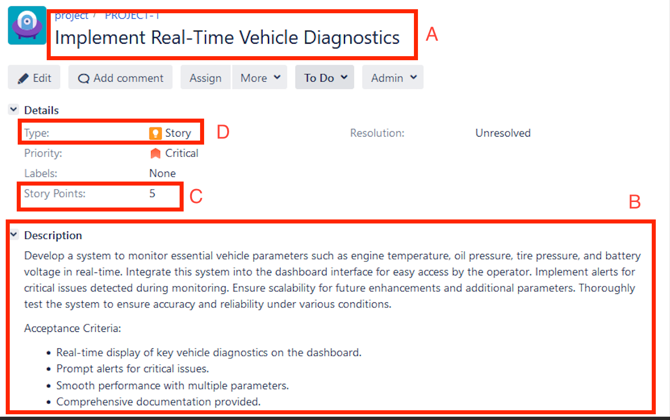
\includegraphics[width=\textwidth]{./figures/dummy-ticket}
        \caption{Example ticket}
        \label{fig:ticket}
    \end{figure}

    The dataset has two types of tickets, ones that have been estimated with a specific time and ones that have been estimated with story points.
    Ones that have been estimated with a specific time also have the ``Actual time spent'' logged on them.
    This is useful as it may help our model become more accurate than a person estimating them, as we can use true values. \par
    An example story point estimation is shown in figure~\ref{fig:ticket}, in box C.
    The projects for this were chosen by looking at projects that have more than 1000 tickets with story points, this is because it is likely that the more tickets that a team has estimated, the more accurate they are at estimating.
    Another requirement was for the tickets to be written only in English, this is because most large language models are language specific.


    \section{Pre-Processing}\label{sec:preprocessing}

    The main features of each ticket is its summary and description.
    The description is written with Jira Markdown syntax, for example it allows formatted blocks of code to be added with the syntax `\{code:java\} \{code\}` and `h[1-6].` formats the following text as a heading.
    In order to remove this syntax and reformat the text as plain text, a set of regex replace rules were used.
    These rules removed blocks of code and formatting syntax, but also has anonymized the data by removing mentions of users, for example `@KatieMaison`.
    This stops the model learning to differentiate the estimation for the ticket by a user as a feature, as this may have ethical considerations. \par
    As mentioned in the ethical considerations section \ref{cha:ethical considerations}, I also tried to remove the risk of gender bias by replacing gendered pronouns with gender neutral pronouns.
 This technique is referred to as Gender Rewriting and is suggested by Rarrick et al in ``Evaluating Gender Bias in the Translation of Gender-Neutral Languages into English
'' which suggests a gender rewriting model based on GPT \cite{rarrick2023evaluating}. However as there were less than 50 occurences of gendered pronouns in the dataset, I performed the rewriting manually.
    Although the paper highlights the difficulty or replacing gendered nouns such as ``mother'' and ``Sister'', it is not common for these words to be used in tickets, and I did not find any in the dataset.
    The method documents a table of gendered pronouns and their respective gender neutral alternatives, for example replacing ``she'' with ``they'' and ``his'' with``theirs'', so I used this for my find and replace.
    The full table of replacements can be found in appendix \ref{ch:appendix}, in table \ref{tab:pronoun_cats}.

    The text string used as an input to the model is the summary prepended to the description.
    This is because usually in a ticket, a title has the most important information in it, often containing keywords about the contents of the ticket. \par
    This is important as the model has a word limit of 512 tokens, and the description is sometimes longer than this, therefore as the description is truncated, the more important information from the summary goes at the start..

    To enable classification, an additional column $class$ was added to the dataset, where $class(ticket) \in \{0,1,2\}$, where 0 is small, 1 is medium and 2 is large.
    ``Small'' tickets have been defined as those that take 1 hour or less to complete and are estimated to be 1 or less Story Point in effort.
    ``Medium'' tickets have been defined as those that take between 1 and 5 hours, or are estimated to be between 1 and 5 story points.
    ``Large'' tickets are defined to take more than 5 hours to complete, or have more than 5 story points as an estimate.

    These classes were chosen as they are the most even split of the data, with 31\% of tickets being small, 37\% being medium and 32\% being large. I chose not to add a fourth class for ``Huge'' tickets as there were very few tickets that were estimated to be 40 or more story points, and the model would not have been able to learn from them effectively.

    The data was then split into a training set and a test set, with 80\% of the data being used for training, 10\% for validation and 10\% for testing.
    The training set is the set of data used to fine tune the model by adjusting the weights of the model so that it can classify the tickets accurately.
    The validation set is used to tune the hyperparameters of the model, such as the learning rate and the batch size as described in section \ref{sec:hyperparameters}, and also .
    The test set is used to evaluate the model, and is not used in the training process.
    The test set and validation set were seperated rather than just using a test set as the model may be overfit to the validation set by the selection of the model and hyperparamaters being based only off the validation set, so the test set can be used to evaluate the model on unseen data.
    The data was split using a stratified split, which ensures that the distribution of classes in the training, validation and test sets are the same as in the original dataset.
    There is also a final unseen data set that is from an unrelated seperate company projects tickets, this is used to evaluate the models performance on tickets that are different in topic and style to the training data. This is described in section \ref{sec:results}.


%\begin{tabular}{|p{7cm}|p{2cm}|p{1.5cm}|p{1cm}|}
%  \hline
%  Ticket Description & Story Point Estimate & Time Logged & Class\\
%  \hline
%  As part of the AUTOSAR project, we need to implement the Controller Area Network (CAN) communication module. This module will facilitate communication between various electronic control units (ECUs) within the vehicle.
% & 5 & N/A & 1 \\
%    \hline
%
%  Row 2, Col 1 & Row 2, Col 2 & Row 2, Col 3 & c2 \\
%  \hline
%\end{tabular}


    \section{Data Augmentation}\label{sec:data-augmentation}
    In order to increase the generalisation of the model and therefore increase accuracy on unseen data, I have opted to use data augmentation to increase the number of data points.
    Back translation was tested as an augmentation technique, this is where a ticket is translated into a different language, and then translated back.
    I used the NLPAug Python library, which allows you to choose a translation model from huggingface to use to translate the text~\cite{ma2019nlpaug}.
    Upon inspecting the tickets, there was very little change in the wording of the ticket, and the model over-fit much more quickly, reaching a very small loss and test accuracy stagnated.
    Instead, paraphrasing had better results.
    To do so, I used a pretrained model from the huggingface library, ``Finetuned ChatGPT paraphraser on T5-base'' \cite{chatgpt_paraphraser}.
    This model is fine-tuned on a dataset of phrases and paraphrases.


    I first used the data cleaner described previously to remove the formatting syntax, then ran the paraphraser on every ticket, generating a single paraphrased version per ticket.
    This took 21 hours on a NVIDIA RTX a4500 Graphics card. An example of paraphrased text is in table \ref{tab:paraphrased} \par
    \begin{table}
    \centering
    \begin{tabular}{p{2.5cm}p{9cm}}
    \toprule
    Original    & As part of ensuring compliance with safety regulations, we need to enhance the safety checks within the critical system.
    This involves reviewing existing safety protocols, identifying potential vulnerabilities, and implementing robust measures to mitigate risks effectively. \\\addlinespace[0.5em]
    Paraphrased & To ensure compliance with safety regulations, we must perform additional safety checks within the critical system. The process entails examining current safety protocols, identifying potential weaknesses, and implementing effective risk mitigation measures.

      \\
    \bottomrule
    \end{tabular}

    \caption{Example of a paraphrased ticket}
    \label{tab:paraphrased}
    \end{table}


    \section{Architectures}\label{sec:architectures}
    The architecture of the model can be described in three parts, Tokenization Layer, Transformer Layers and Classification Head.
    These will be described sequentially in the following sections and is shown in figure \ref{fig:model-architecture}.\par

    \begin{figure}[h]
        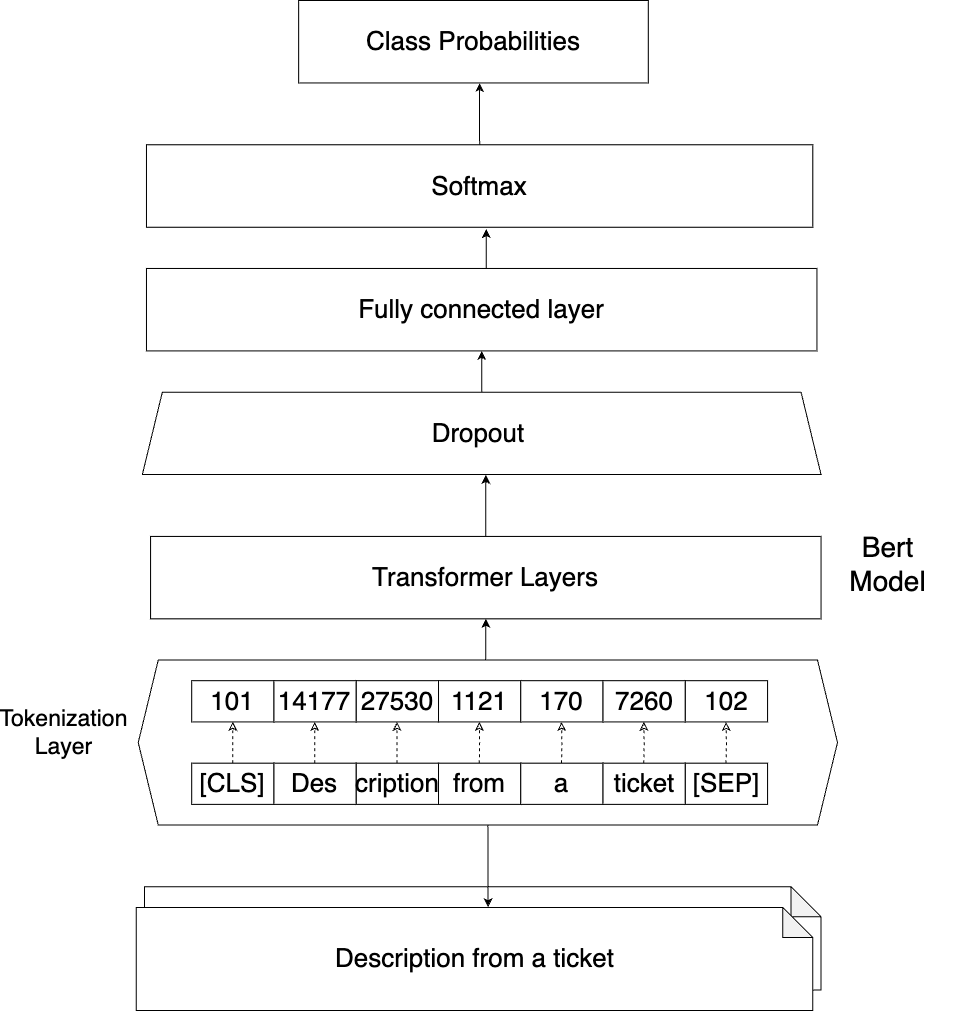
\includegraphics[width=\textwidth]{./figures/testmodel}
        \caption{Model Architecture}
        \label{fig:model-architecture}
    \end{figure}

    \subsection{Tokenization Layer}\label[tokenization-layer]
    In order to be used in a Large Language Model, textual input needs to be transformed into tokens and embeddings.
    My model uses the BERT Tokenizer, the specific implementation of which is provided by the transformers huggingface library. \par

    \begin{figure}[h]
        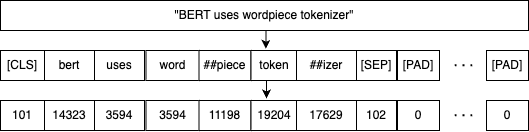
\includegraphics[width=\textwidth]{./figures/tokenizer-example}
        \caption{Bert Tokenizer Example}
        \label{fig:tokenizer-figure}
    \end{figure}

    % Maybe i can add to the tokenizer vocab? https://medium.com/@pierre_guillou/nlp-how-to-add-a-domain-specific-vocabulary-new-tokens-to-a-subword-tokenizer-already-trained-33ab15613a41
    The tokenizer works by splitting each tickets description into individual tokens, then converting these into a numerical value from the models vocabulary.
    As shown in the example in figure~\ref{fig:tokenizer-figure}, tokens can be a single word, or a sub-word, or a character. The tokenizer breaks down the text into these tokens based on what is in its vocabulary.
    In the example, the word ``tokenizer'' is split into ``token'' and ``\#\#izer'', as the word ``tokenizer'' is not in the vocabulary, but the sub-word ``token'' is.
    The special token [CLS] is added to the start of the tokenized text, and [SEP] is added to the end, and between sentences if there are multiple in one input.
    The end of the tokenized text is then padded with [PAD] tokens to the length of the limit of the model, which is 256.
    The tokens are then padded to the length set, in this case 256 and then the tokenized test is passed to the transformer layers.
    The BERT Tokenizer used is uncased, meaning that it turns everything into lower case and removes accents before tokenizing it.
    \par

    One of the benefits of the preprocessing discussed in section~\ref{sec:preprocessing} is that it reduces the size of the textual description in the dataset, as it removes a lot of characters.
    This enables the model to get more information from the text, as the model has a word limit of 256 tokens. As each non-alphanumeric character is a token in iteself, this means that the model can get more information from the words in the text once these are removed.
    I tokenized the data before and after preprocessing, and found that the average number of tokens in the description was reduced from 111 to 91. The upper quartile value and upper range was also reduced to fall inside the 256 token limit.
    This is shown in figure~\ref{fig:token-boxplot}.

    \begin{figure}[h]
        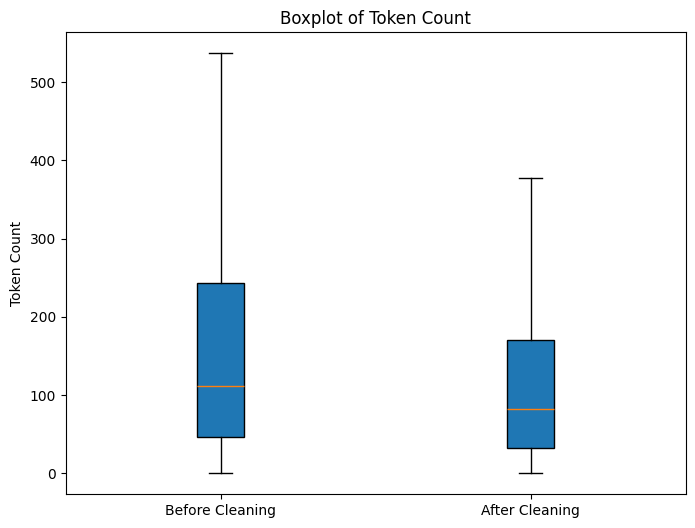
\includegraphics[width=\textwidth]{./figures/tokencount-prepost}
        \caption{Boxplot showing statistics on the number of tokens in the description before and after preprocessing.}
        \label{fig:token-boxplot}
    \end{figure}


    \subsection{Transformer Layer}\label{subsec:Transformer-Layer}
    The transformer layers are the core of the model, they are the part of the model that is responsible for understanding the context of the tokens.
    A transformer layer is a type of neural network architecture that is designed to process sequential data, such as text, and is based on the concept of attention.
    In a transformer layer, the input is passed through multiple layers of attention and feed forward neural networks.
    As previously discussed, the transformer architectures self attention mechanism allows the capturing of long-range dependencies and contextual information.
    After obtaining contextualized representations through self-attention, the outputs are passed through a feed-forward neural network (FFN).
    This network applies linear transformations and non-linear activation functions to capture complex patterns and relationships within the representations.
    The FFN enables the model to distill and refine the contextual information obtained from self-attention, producing richer and more informative representations of the input sequence.
    In the context of this model, I have experimented with multiple pretrained BERT models that use the transformer architecture that have various benefits, including optimization of training time and size.
These are explained in more detail below. \par
    The pretrained model is then fine-tuned on the dataset, where it learns the specific context of the tickets in the dataset.

    \par

    \textbf{BERT Base Uncased: Bidirectional Encoder Representations from Transformers}

    This model is the original weights for the pre-trained BERT model, with 12 transformer layers, each with 12 attention heads.
    It is downloaded from the huggingface model hub, and is the most widely used BERT model~\cite{bert-base-uncased}.
    \par

    \textbf{BERTOverflow: Code and Named Entity Recognition in StackOverflow}
    BERTOverflow is a BERT model that is pre-trained on a large corpus of 152 million sentences from StackOverflow, a question and answer website for programming questions~\cite{tabassum2020code}.
    Although the architecture of this model is the same as the classic BERT model, the fine-tuning is expected to enable the model to better understand the context of the text.
    \par

    \textbf{DistilBERT: a distilled version of BERT: smaller, faster, cheaper and lighter}
    DistilBert is a smaller version of BERT, it has 6 transformer layers, each with 12 attention heads.
    It is trained using knowledge distillation, a process where a smaller model is trained to mimic the outputs of a larger model.
    This is done by training the smaller model to predict the outputs of the larger model, rather than the ground truth.
    This allows the smaller model to learn from the larger model, and therefore be more efficient.
    DistilBERT is 40\% smaller than BERT and is 60\% faster~\cite{sanh2020distilbert}.
    \par

    \textbf{ALBERT: A Lite BERT for Self-supervised Learning of Language Representations}
    ALBERT is a ``lite'' version of BERT, it is 18x smaller and 1.7x faster than BERT.
    It is trained using a cross-entropy loss, rather than the masked language model objective used by BERT.
    This is because the masked language model objective is computationally expensive, as it requires the model to predict the probability distribution over all tokens in the sequence.
    ALBERT uses a factorized embedding parameterization, which reduces the number of parameters in the model.
    This is done by decomposing the large vocabulary embedding matrix into two smaller matrices~\cite{sanh2020distilbert}.
    \par

    \subsection{Classification Head}\label{subsec:Classification-Head}
    The output of the transformer model is then passed into a fully connected layer.
    This maps the contextual embeddings that are output to predictions for each of the 3 classes in the classification task in question.
    This means that it transforms from a $1\times768$ sequence which is the output fromm a BERT model, to an output vector of dimension $1\times3$ by
    Each value in the output vector represents the score for one of the classes.
    Softmax is then used to normalise the values in the vector to sum to 1, such that the values can be interpreted as probabilities \cite[p.~809]{russel2010}.

    The classification head uses Cross Entropy Loss to calculate the difference between the models output probability and the ground truth.
    The loss function is defined as:
    \[-\sum_{c=1}^My_{c}\log(p_{c})\]
    Such that $y_{c}$ is the ground truth label for class $c$, and $p_{c}$ is the predicted probability for class $c$.
    The ground truth is represented as a probability density function of a Guassian Distribution such that the vector representing the label of a ticket $l$ is calculated with:

    \[f(x) = (1-\frac{1}{\sigma \sqrt {2\pi}}) \times e ^{-\frac{1}{2}(\frac{x-\mu }{\sigma})^{2}}\]

    where $\mu$ is the mean of the class, in this case it is the target label, $x$ is a vector representing the labels of the class. ie. $[0,1,2]$ for a 3 class problem as in this model .
    $\sigma$ is the standard deviation of the distribution.
    This value is between 0 and 1, and adjusts the spread of the values in the vector for the ground truth.

    This loss function was chosen as it takes into consideration the sequential nature of the labels as labels that are closer to each other on the sequence (e.g., 0, 1, 2 for this 3-class problem) will have higher probabilities assigned to them, reflecting the sequential nature of the classes.

    \section{Hyperparameters}\label{sec:hyperparameters}
    In order to decide on a learning rate and batch size, I performed a grid search.
    The grid search was performed on the base bert model, and the best parameters were chosen based on the testing accuracy.
    The original bert paper suggests the following hyperparameters:
    \begin{itemize}
        \item Batch size: 16, 32
        \item Learning rate (Adam): 5e-5, 3e-5, 2e-5
        \item Number of epochs: 2, 3, 4
    \end{itemize}
    Each combination of learning rate and batch size was trained for 20 epochs, and the best performing model was chosen.
    However, Mosbach et al. researched the instability of fine tuning BERT and found that the number of epochs should be considerably higher and that using a small learning rate with bias correction helps to avoid vanishing gradients early in training, whereby the gradients become so small that the model stops learning~\cite{mosbach2021stability}.
    Therefore, I used the Adam optimizer to train the model, as this is the optimizer that is used in the original BERT paper and is also suggested in Mosbach et al.
    The learning rate also linearly increased for the first 10\% of steps, as suggested by Mosbach et al. again, to avoid vanishing gradients.
    This was done using the transformers library implementation of linear scheduling with warmup~\cite{transformerLinearSchedular}.
    The learning rate was then decayed by a factor of 0.01 which is the default for the Pytorch implementation of the Adam optimizer~\cite{adamPytorch}.

    The model was trained on a NVIDIA RTX 4500, and took approximately 6 hours to train for 30 epochs. \par

    The model was trained on the training set, and then evaluated on the validation set.
    The training and validation set were explained further in section \ref{sec:preprocessing}.
    The model was evaluated using the accuracy metric, which is the number of correct predictions divided by the total number of predictions.
    It was also evaluated using the F1 score, which is the harmonic mean of precision and recall.
    Where precision is the number of true positives divided by the number of true positives and false positives, and recall is the number of true positives divided by the number of true positives and false negatives.

    To enable me to find the best model, I tested the model on the validation set after every epoch.
    I then made a record of the results for each epoch and chose the model with the best accuracy and F1 score.
    As the number of epochs is much smaller than traditional neural networks, early stopping was not used.
    Particularly as I found the model to be quite stable, and the loss to decrease consistently over the 30 epochs.

    I found that the model performed best with a batch size of 32, and a learning rate of 3e-5.
    It achieved a validation accuracy of 0.7330 and a F1 score of 0.7332 after 20 epochs.

    \chapter{Experimental Model Evaluation}
    \label{ch:experimental-model-evaluation}
    This chapter discusses the results of training the different bert models on the dataset.
    The results of these experiments were used to decide whether there are any significant differences between the models, and which model is the best to use for the final model.

    \section{Accuracy evaluation}\label{sec:accuracy-evaluation}
    All models were trained for 30 epochs, as despite the hyperparameter search finding the best accuracy at 20 epochs, I did not want to limit the epochs because time to train is more important to reduce cost than number of epochs.
    The best accuracy on the validation set was taken after testing on every epoch and the results are displayed in table~\ref{tab:accuracy} and figure ~\ref{fig:accuracy}. \par

%    \setlength{\tabcolsep}{4ex}
    % increase row space
% \usepackage{graphicx}
% \usepackage{booktabs}


\begin{table}[h]
\centering
\begin{tabular}{ccccc}
\toprule
Model        & Accuracy & F1     & Epochs  & Time to Train\\
\midrule
Bert Base    & 0.7330   & 0.7332 & 20 & 380 minutes     \\\addlinespace[0.5em]
DistilBert   & 0.7189   & 0.7192 & 25 & 240 minutes     \\\addlinespace[0.5em]
Albert       & 0.7061   & 0.7075 & 29 & 464 minutes    \\\addlinespace[0.5em]
BertOverflow & 0.7103   & 0.7114 & 2 & 392 minute      \\
\bottomrule
\end{tabular}

\caption{Accuracy of models} \label{tab:accuracy}
\end{table}

\begin{figure}[h]
    \centering

        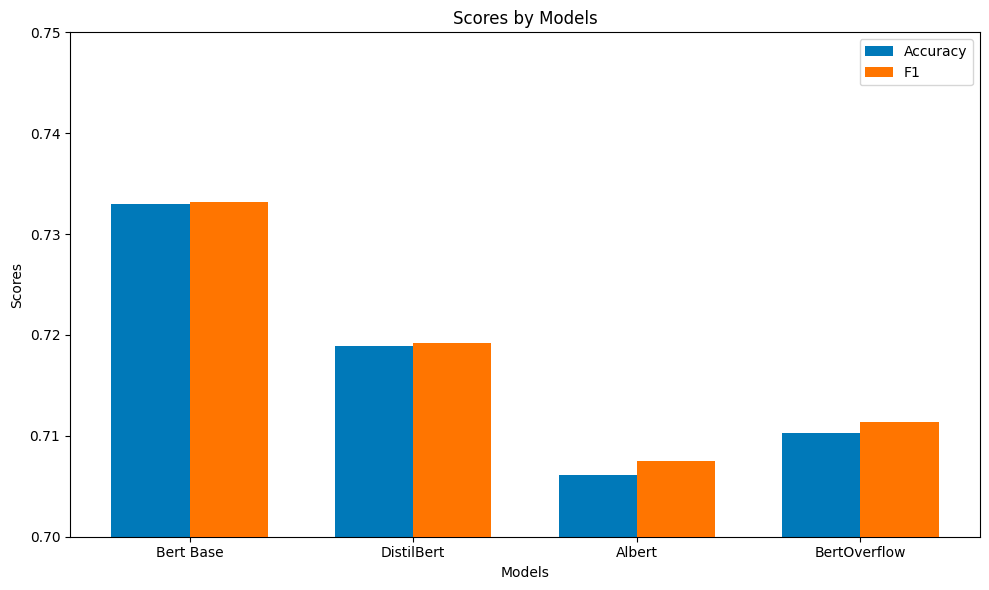
\includegraphics[width=12cm]{./figures/model-accuracy}
        \caption{Bar chart showing the accuracy of the models}
        \label{fig:accuracy}
    \end{figure}

    The Bert-base-uncased model performed the best, followed by the Distilbert model.
    Distilbert was faster to train than the Bert-base-uncased model, taking 240 minutes to train for 25 epochs, compared to 380 to train for 20 epochs.
    This would mean that the Distilbert model would be more cost effective to train, as it would take less time to train.
    However it is less accurate, so a trade-off would need to be made between accuracy and cost.
    Time to train is particularly important in the context of this project, as the model is likely to be retrained on a regular basis, as the data is regularly changing and more datapoints are being added.
    Cost is also important, as the model is likely to be trained on a cloud service, and therefore the cost of training the model is likely to be high, and billed per minute.

    The Albert model performed the worst, with an accuracy of 0.7061, and a F1 score of 0.7075 and took the longest to train, at 464 minutes for 29 epochs.
    However the graph of the accuracy in figure~\ref{fig:accuracy-graph} shows that the models accuracy on the validation set was still increasing, and therefore it may have performed better with more epochs.
    The graph also shows that the BertOverflow models accuracy steadily decreased after 2 epochs, and therefore it is likely that the model was overfitting the training data, particularly as the loss value continued to get smaller.
    However it appears that after 23 epochs, the accuracy starts to increase again, suggesting that the model may have started to generalise more effectively and may have continued increasing in accuracy if trained for longer.
     \par

\begin{figure}[h]
    \centering

        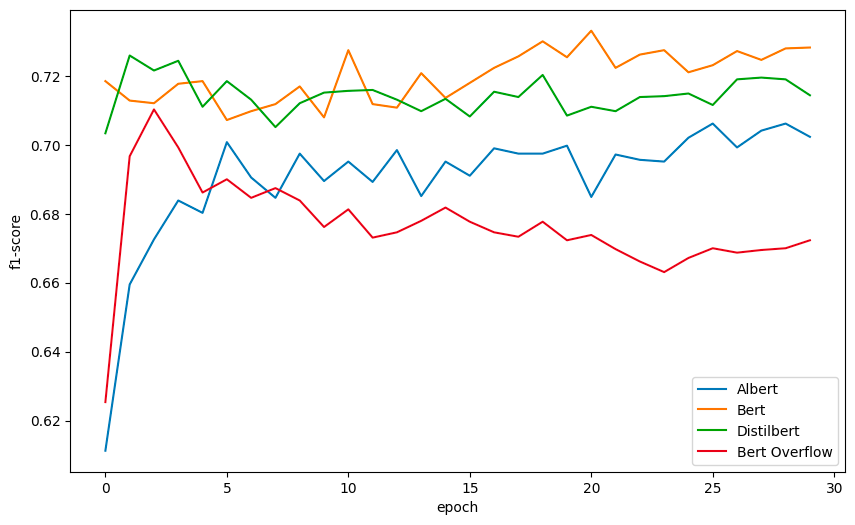
\includegraphics[width=10cm]{./figures/accurach-epochs}
        \caption{Graph showing the accuracy of the models over the number of epochs on the validation set}
        \label{fig:accuracy-graph}
    \end{figure}

    \chapter{Finalised Model and Results }
    \label{ch:results}

    This chapter discusses the final model, and the results of testing the model on the test set.
    It also discusses the results of testing the model on a different unrelated project, to see how well the model generalises to unseen data.
    Finally I perform an ablation study to see how well the model performs without the paraphrased data, custom loss function and data preprocessing.


    \section{Results}\label{sec:results}
    The final model was trained on the entire dataset, and then tested on the test set after 20 epochs.
    This test set was not used in the training of the model but is from the same projects, and therefore is a good representation of how the model will perform on unseen but related data.
    I then tested it on a set of tickets from a different project, to see how well it generalised to unseen data that is more likely to be different from the training data.

    A seperate test set was used rather than using the validation set.
    This is because the validation set was used to compare the models, and therefore the model may have been overfit to the validation set.
    When using the test set, the model achieved an accuracy of 0.7348 and an F1 score of 0.7368.
    It took 3 hours and 45 minutes to train the model without testing at every epoch unlike the times in the previous chapter.


    The results show that the model performs better on the classes for small and large, and worse on the medium class.
    This is likely due to the fact that the medium class is the most ambiguous, and therefore the hardest to classify, even for a human.
    The confusion matrix in table~\ref{fig:confusion-matrix} shows that the model is able to capture the sequential nature of the classes, as the model is more likely to predict a ticket as a class that is closer to the actual class.
    This is shown by the fact that the model is more likely to incorrectly predict a small ticket (0) as being a medium ticket (1) than a large ticket (2).

    In terms of where it fits in the literature, the model is more accurate than the model proposed by Choetkiertikul et al. \cite{8255666} however Choetkiertikul uses a Standardised Accuracy score because it estimates a specific value rather than a class, as desscribed in section \ref{sec:estimation-with-deep-learning}, which classifies tickets up to 71\% accuracy.
    A more relevant comparison is with the model proposed by Phan et al. \cite{phan2022story}, which achieved an average accuracy of 78.63\% over all the projects in their dataset, when classifying tickets into 4 classes.
    This is higher than the model proposed in this paper, however the model in this paper is is shown to be effective at classifying tickets across multiple projects in a company rather than just a single project per company, so therefore may generalise better.

\begin{table}
\centering
\begin{tblr}{
  cells = {c},
  cell{1}{2} = {c=4}{},
  cell{2}{1} = {r=4}{},
  vlines,
  hline{1-2,6} = {-}{},
  hline{3-5} = {2-5}{},
}

                                            & Predicted Labels &     &     &     \\
\begin{sideways}Actual Labels\end{sideways} &                  & 0   & 1   & 2   \\
                                            & 0                & 442 & 242 & 32  \\
                                            & 1                & 207 & 753 & 192 \\
                                            & 2                & 34  & 218 & 541
\end{tblr}
\caption{Confusion Matrix for final model on test set.}\label{fig:confusion-matrix}
\end{table}
    The model was then tested on a different project. The project tested is for a plaform team, that mostly creates automations and cloud resources which is very different to the automotive projects in the training data.
The model achieved a 44.2 \% accuracy on the project.
We can compare this to the accuracy of randomly guessing the values by calculating the weighted probability of each class, using the class sizes discussed in section \ref{sec:preprocessing}.
The accuracy of randomly guessing the values is 0.335. This means that the model is 9\% more accurate than randomly guessing the values.
    This shows that the model does not perform well on a different project, and therefore the model may not generalise well to unseen data that is unrelated to training data.

    To compare the model to human estimation accuracy, I used the set of tickets that had been estimated with a specific time and that had an actual time documented to compare to.
    I then placed the estimated and actual time into the same categories as for the model, small, medium and large.
    From this I was able to calculate the accuracy of the model, and the results show that the human accuracy is 0.77.
    This is 3-4\% higher than the model.
    However, as the model is trained on tickets throughout the entire history of the project, the model is able to estimate tickets that are similar to ones that have been estimated before, and therefore the model is able to learn from the history of the project, rather than just the tickets that have been estimated or worked on by the person, or people, estimating the tickets.
    This may mean that when a type of ticket hasnt been seen for a long time, the model may estimate it more accurately than a person who may not remember the details of the previous similar ticket.
    However this is difficult to test as pairing tickets from the same project that are similar is difficult and would require a deep understanding of the project, so would need to be done by a team member.

The time taken to estimate the tickets was also examined, and the model was able to estimate the tickets on average in 0.009 seconds per ticket when running on the machine that it was trained on as described in \ref{sec:hyperparameters}.
This was tested by estimating each ticket in the test set, including time taken to use the jira Markdown syntax remover and tokenise the data.
The range was between $9 \times 10 ^{-4}$ and 0.14 seconds.
This is much faster than a human, who would need to take time to read the ticket and understand the context of the ticket before estimating it.
In a production system, the time that the model would take may be affected by the hosting solution, as discussed further in \ref{ch:practical-application}.

    \section{Ablation Study}
    In order to see how much the paraphrased data, custom loss function and data preprocessing helped the model, I removed each in turn, testing the model on the test set after each change and also the unseen data from a seperate project.

    The results of these tests are shown in table~\ref{tab:accuracy-ablation} \par

\begin{table}[h]
\centering
\begin{tabular}{ccc}
    \toprule

                     & Accuracy   & F1         \\
    \midrule
No Data Augmentation & 0.6485 & 0.6302 \\
No Pre Processing    & 0.7164 & 0.7175 \\
No Gaussian Labels   & 0.7249 & 0.7249 \\
Original             & 0.7348  & 0.7358 \\
    \bottomrule
\end{tabular}
    \caption{Accuracy of ablation study} \label{tab:accuracy-ablation}

\end{table}

    I first trained the model on the original dataset without adding the paraphrased data. The aim of this is to see if the model performs better with the paraphrased data or if the paraphrasing is too different from the original data and it doesnt help, or if the data is too similar and overfits.

    The results show that the model performs better with the paraphrased data.
    This is likely because the paraphrased data allows the model to see more examples of different ways that tickets can be written, and therefore the model is able to generalise better to unseen data.
    \par
    I then trained the model on the original dataset without using Gaussian Distribution as the label for cross entropy loss.
    This is to see if the custom loss function helps the model to learn the sequential nature of the classes.
    The results show that the model performs better with the custom loss function, despite only a small improvement, it enables the model to have a more useful output, as the model is more likely to predict a ticket as a class that is closer to the actual class. This is shown by the comparison of the confusion matrix in figure~\ref{fig:confusion-matrix} and the confusion matrix in figure~\ref{fig:confusion-matrix-no-guassian} [TODO]. The no guassian models confusion matrix shows a slightly wider spread of values. This means for example, that when a ticket is small, the guassian model is more likely to predict it as medium, rather than large, than the no guassian model is.
    However it is only a small improvement, and therefore the model may be able to be simplified by using the standard cross entropy loss function. \par

    I then trained the model on the original dataset without using the data cleaner, which removes the Jira markdown syntax from the text as described in \ref{sec:preprocessing}.
    This is to see if the data cleaner helps the model to learn the context of the tickets, or if context is lost in the cleaning process.
    The results show that the model actually performed almost the same without the data cleaner.
    Although the datacleaner removes syntax and allows more of the text of the description to be used, which I expected to have a large effect on the accuracy, it may be that the model is able to learn from the syntax in relation to the context of the ticket.
    Further experiments could be done to see if the data cleaner is actually needed, or if the model can learn the context of the ticket without it given more fine tuning and potentially more data.






    % Test with a validation set and then a test set from a different project and also unseen tickets from the same project




    % Add a table of results
    % Test final model on unseen projects data and compare to previous models



    \chapter{Practical Application}
    \label{ch:practical-application}

    In order to contextualise the model, in this section I have proposed a way that an organisation could use the model, and discussed how the model could be used in a software development team.
    \section{Model as a service}\label{sec:model-as-a-service}

In order for an organisation to benefit from the model proposed, the model would need to be hosted as a service, and integrated into the organisations workflow.
The model would need to be specific to an organisations projects, as the model would need to be trained on the organisations data in order to be able to estimate the size of the tickets.
This would mean that the model would need to be trained on the organisations data, and then deployed as a service that the organisation could use to estimate the size of the tickets.
An organisation may even need multiple models that are trained on different catagories of tickets, for example one model for frontend tickets, and one model for backend tickets.
This would allow the model to be more accurate, as the model would be able to learn the context of the tickets better, and therefore be able to estimate the size of the tickets more accurately.
As demonstrated with the testing of unseen tickets in an unrelated project, the model does not generalise well to unseen data that has a different topic, and therefore the model would need to be trained on subsets of the organisations data in order to be able to estimate the size of the tickets.

    In practice, this would be done by the addition of a button in Jira that estimates the ticket via an automation.
Once the user has input the title and description of the ticket, they would click the button, and the model would estimate the size of the ticket.
A user would then be able to edit the description, and when ready, they would click the ``Estimate' button, and the model would re-estimate the size of the ticket.
    The model would need to be hosted, this could be done on a cloud service such as AWS, or on a local server.
In AWS the model could be hosted on a SageMaker instance, which is a managed service that allows you to train and deploy machine learning models.
This would allow the model to be easily scaled to meet the demands of usage of the model, and would also allow the model to be easily updated with new data.
The cost of hosting the model would depend the amount of traffic that the model receives.
The model would also need to be trained on new data regularly, as the model would need to be updated to reflect the changes in the project.
The cost of maintaining the model may be quite high as a result of this.
A another thing that needs to be taken into account when hosting the model is the response times.
Although the model has an average time to estimate of 0.009, this is just the model itself. Once it is hosted, the time taken for an API response would affected by the hosting solution, the size of the model, and the amount of traffic that the model receives and the network speed.
Testing this is outside the scope of this paper, but would be important to do before deploying the model to a production system.
%TODO: add a diagram of the cloud hosting?

    \section{Use in a software development team} \label{sec:use-in-a-software-development-team}
    One proposed way that a team would use this model is during a planning poker session.
    As previously discussed, planning poker is a technique used in agile software development to estimate the size of a user story or task.
Planning poker often involves the team discussing the size of the ticket, and then voting on the size of the ticket.
    The model could be used to give a pre-estimate of the ticket, and then the team could use this as an addition point for their discussion.
It may also be beneficial to use the model to estimate the size of the ticket before the planning poker session and instead of outputting a single class, output a probability distribution over the classes.
    This would allow the team to see how confident the model is in its prediction, and therefore the team could use this as a guide to prioritise tickets where the model is less confident in its prediction, as these may require more in depth discussion.
    However, in this scenario, we must be careful of anchoring bias.
    Whereby the first answer given to a person acts as an 'anchor' and they are more likely to give an answer close to the anchor.
    This is researched in multiple fields, including medicine, where doctors are more likely to give a diagnosis close to the first diagnosis they hear~\cite{biasMedicine}.
This has also been researched in software development, where it is found that developers are more likely to give an estimate close to the first estimate they hear~\cite{softwareBias}.
    As a result of this, it may be more suitable to show the estimation to developers after they have made their estimations and had a discussion to avoid anchoring bias.


    \chapter{Conclusion and further work}
    \label{ch:conclusion}

    In this paper, I have proposed a model for the classification of software development tickets into 3 classes, small, medium and large.
    The model uses a BERT model, and is trained on a dataset of 19,500 tickets from 7 projects.
    The model is able to classify the tickets with an accuracy of 0.7348, and an F1 score of 0.7358.
    This means that it is able to classify the tickets with an accuracy of 73.48\%.
    This is almost as accurate as a human, who has an accuracy of 77\%.
In terms of usefulness, unfortunately the model does not generalise so well to tickets from projects it has never seen before.
    This is likely due to the fact that each project has its own way of writing tickets, different paces of work and different topics, and therefore the model is not able to predict the size of the ticket without seeing the projects tickets previously.
    This means that this model would only be useful for particular projects with enough history to train the model, and therefore the model is not suitable to be used for new projects.
    In terms of the 3 objectives of the project as listed in the introduction in section \ref{sec:introduction}, the model is able to estimate the size of the tickets out of the three options listed with an accuracy of 73.48\%, which fulfills objective 1. The final model took 3 hours and 45 minutes to train, which is within the time limit of 4 hours, and therefore fulfills objective 2. The model is able to estimate the size of the tickets in 0.009 seconds, which is within the time limit of 0.01 seconds, and therefore fulfills objective 3. It is currently unclear how the model would perform in a production system, as this was not tested in this paper, and therefore as previously discussed in section \ref{sec:model-as-a-service}, further work would be needed to see how the model performs in a production system.

    Another limitation of the model is that it has only been trained on text written in English. This means that the model is not able to classify tickets that are written in a different language, and therefore the model is not suitable for projects that are not written in English.
    However, an option for further work would be to train the model on tickets written in different languages, and then use a language detection model to determine the language of the ticket, and then use the appropriate model to classify the ticket. Alternatively, one could use a model that is trained on multiple languages, such as mBERT, which is a multilingual version of BERT. This model is trained on 104 languages, and is able to understand the context of text in multiple languages~\cite{devlin2018bert}. However, this model is much larger than the models used in this paper, and therefore would be more expensive to train and use.

    A further limitation of the model is that it is not able to estimate the time that a ticket will take to complete, only the size of the ticket. An option for further work would be to train the model to predict the actual story point or time values rather than the size of the ticket. This would be more useful for the team, as they would be able to see how long a ticket will take to complete, rather than just the size of the ticket. This would be particularly useful for projects that have deadlines and releases to meet, as the team would be able to see how long each ticket will take to complete, and therefore be able to plan their work more effectively.

    The model would be most beneficial to projects that have new team members, or team members that are not experienced in estimating tickets. This is because it can use the history of the project to estimate the size of the ticket, and therefore the team members can act as a sanity check in the estimation process. For example if a user estimates a ticket as small, but the model estimates it as large, the team may be more likely to investigate the ticket further, and therefore the model can be used as a tool to help the team estimate the tickets more accurately. This would be particularly useful for projects that have a large number of tickets, as the model could be used to give pre estimates before the ticket goes through the formal human estimation process, allowing the team to focus on estimating larger tickets if they have lots of spare capacity that requires larger tickets to be ready to implement, or smaller tickets if they have less capacity.





\appendix
\chapter{Appendix}\label{ch:appendix}

\begin{table*}[!ht]
\centering
\begin{tabular}{llll}
\toprule
Category & Feminine & Masculine & Neutral \\
\midrule
Subject & She & He & They \\
Object & Her & Him & Them \\
Possessive Determiner & Her & His & Their \\
Possessive Pronoun & Hers & His & Theirs \\
Reflexive & Herself & Himself & Themselves \\
\bottomrule
\end{tabular}
\caption{Pronoun categories \cite{rarrick2023evaluating}}
\label{tab:pronoun_cats}
\end{table*}



\printbibliography

\end{document}
